%! Author = michael
%! Date = 08.10.20

% Preamble
\documentclass[11pt]{article}
\usepackage{pdfpages}
\usepackage[german]{babel}
\usepackage{amsmath}
\usepackage[backend=biber]{biblatex}
\usepackage{csquotes}
\usepackage{changepage}

\setlength{\parindent}{0em}
\setlength{\parskip}{0.8em}

\addbibresource{main.bib}

% Document
\begin{document}
    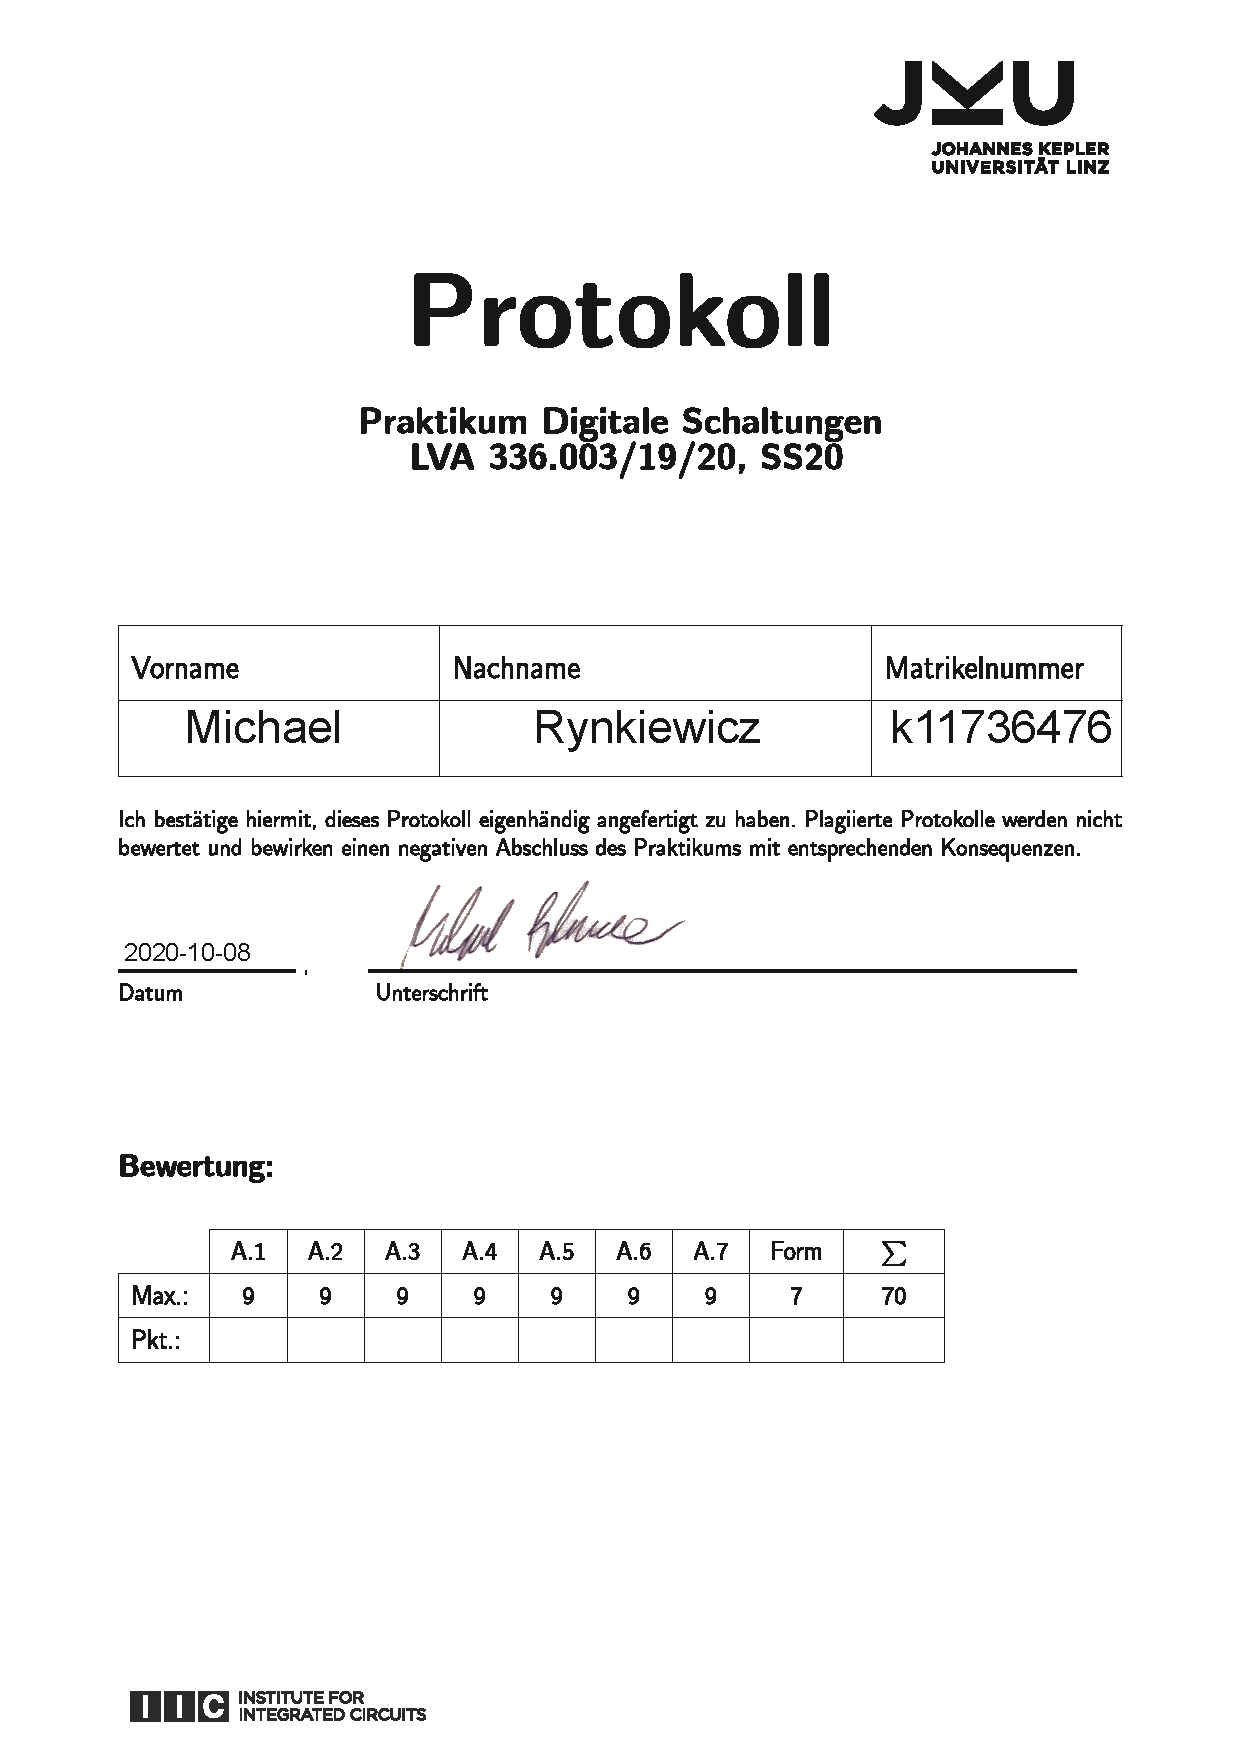
\includepdf[pages=-]{deckblatt.pdf}

    \tableofcontents
    \newpage


    \section{Einleitung}
    \label{sec:einleitung}

    Das Wissen um die Funktionsweise eines Mikrocontrollers ist wesentlicher Bestandteil eines Informatik-Studiums.
    Im Zuge Dieses werden in diesem Protokoll verschiedene Experimente beschrieben und evaluiert.
    Insgesamt werden sieben Experimente begutachtet und diskutiert, welche im Zeitraum vom 28.September 2020 und 2.Oktober 2020 durchgeführt wurden.


    \section{Verwendete Materialien}
    \label{sec:verwendete-materialien}

    Jede Sektion gibt die in ihr verwendeten Materialien mitsamt ihrer Stückzahl an.
    In dieser Sektion werden alle Materialien im Allgemeinen gelistet und beschrieben.

    \subsection{LED}
    \label{subsec:led}
    Eine Leuchtdiode (LED) ist ein Bauelement der Elektronik.
    Wird sie von elektrischen Strom durchflossen beginnt sie Licht auszustrahlen.
    Die Wellenlänge, d.h., die Farbe des Lichts sowie ob es für das menschliche Auge sichtbar ist oder nicht, hängt von den benutzten Materialien im inneren der LED ab.
    Die in der LED verwendeten Materialien sind für dieses Protokoll nicht weiter von Bedeutung.
    Für die beschriebenen Aufgaben wurden die folgenden LEDs verwendet.

    \begin{table}[h]
        \centering
        \caption{LEDs - Farben, Flussspannung, Maximalstrom \cite{led-elektrische-eigenschaften}}
        \label{tab:leds-farben-und-elemente}
        \begin{tabular}{| l | l | l |}
            \hline
            Farbe & Durchflussspannung & Maximalstrom \\
            \hline
            Rot   & 1,6V - 2,2V        & 20mA         \\
            Gelb  & 1,9V - 2,5V        & 20mA         \\
            Grün  & 1,9V - 2,5V        & 20mA         \\
            \hline
        \end{tabular}
    \end{table}

    \subsection{Widerstände}
    \label{subsec:widerstände}

    Widerstände werden verwendet, um einen Spannungsabfall in einem Stromkreis zu verursachen.
    Damit kann die Stromstärke in einem Stromkreis begrenzt beziehungsweise verringert werden.
    Oft wird bei der Verwendung von LEDs ein sogenannter Vorwiederstand verwendet, um die Stromstärke soweit abzusenken, dass die LED nicht beschädigt wird.

    In den Aufgaben wurden Widerstände der sogenannten E6-Reihe verwendet.
    E-Reihen sind normierte Widerstandsgrößen, wobei die Zahl die Stufen zwischen den Potenzen angibt.
    D.h., bei der E6-Reihe sind sechs verschiedene Widerstandsgrößen zwischen $10\Omega$ und $100\Omega$, zwischen $100\Omega$ und $1000\Omega$, u.s.w. bis zum oberen Limit von $10M\Omega$.

    Die verwendeten Widerstände sind Farbcodiert, um sie voneinander unterscheiden zu können.
    Die Farbkodierung von Widerständen wird in den Aufgaben, in denen sie verwendet werden, angegeben.
    Die Bedeutung der Codierung der verwendeten Widerstände kann in Tab. \ref{tab:farbcodierung-von-widerständen} abgelesen werden.

    \begin{table}
        \begin{adjustwidth}{-2cm}{}
            \caption{Farbcodierung von Widerständen}
            \label{tab:farbcodierung-von-widerständen}
            \begin{tabular}{| l | l | l | l | l |}
                \hline
                Farbe & 1.Ring (10er Stelle) & 2.Ring (1er Stelle) & 3.Ring (Multiplikator) & 4.Ring (Toleranz) \\
                \hline
                Braun & 1                    & 0                   & 10                     & $\pm 1$           \\
                Grün  & 5                    & 5                   & $100\ 000$             & $\pm 0.5$         \\
                Gold  & -                    & -                   & $0.1$                  & $\pm 5$           \\
                \hline
            \end{tabular}
        \end{adjustwidth}
    \end{table}

    \subsection{Mikrocontroller}
    \label{subsec:mikrocontroller}



    \section{Aufgabe 1 - Ampelsteuerung}
    \label{sec:aufgabe-1}

    Es soll eine Ampelsteuerung implementiert und getestet werden.
    Die Ampel wird mithilfe von drei LEDs, in den Farben Rot, Gelb und Grün, aufgebaut.
    Weiters soll die Steuerung folgende Funktionsweise implementieren:

    \textbf{Phase 1} soll die Ampel auf Rot setzen.
    D.h., die rote LED wird eingeschaltet.
    Dieser Zustand soll vier Sekunden lang gehalten werden.

    \textbf{Phase 2} soll zusätzlich zur roten LED die gelbe einschalten.
    Dieser Zustand soll eine Sekunde lang gehalten werden.

    \textbf{Phase 3} soll die rote sowie die gelbe LED ausschalten, während die Grüne eingeschaltet wird.
    Dieser Zustand soll vier Selunden lang gehalten werden.

    \textbf{Phase 4} soll die grüne LED ausschalten während die Gelbe eingeschaltet wird.
    Dieser Zustand soll eine Sekunde lang gehalten werden.
    Nach Ablauf der vier Sekunden soll die grüne LED erlöschen und der Ablauf bei Phase 1 neu gestartet werden.

    \subsection{Materialien}
    \label{subsec:A1-materialien}

    \begin{table}[h]
        \centering
        \caption{Aufgabe 1 - Verwendete Materialien}
        \label{tab:a1-materialien}
        \begin{tabular}{| l | l | l |}
            \hline
            Bezeichnung & Eigenschaften & Menge \\
            \hline
            Widerstand  & $150\Omega$   & 3     \\
                        & Braun - Grün - Braun - Gold & \\
            LED & Rot & 1 \\
            LED & Gelb & 1 \\
            LED & Grün & 1 \\
            Mikrocontroller & Arduino Uno R3 & 1 \\
            \hline
        \end{tabular}
    \end{table}

    \subsection{Vorbereitung}
    \label{subsec:A1-vorbereitung}

    \addcontentsline{toc}{section}{References}
    \printbibliography
\end{document}
